\documentclass[onecolumn]{article}
\usepackage{url}
\usepackage{algorithmic}
\usepackage[a4paper]{geometry}
\usepackage{datetime}
\usepackage[margin=2em, font=small,labelfont=it]{caption}
\usepackage{graphicx}
\usepackage{mathpazo} % use palatino
\usepackage[scaled]{helvet} % helvetica
\usepackage{microtype}
\usepackage{amsmath}
\usepackage{subfigure}
\usepackage{amssymb}
\usepackage{enumitem} % alphabetic enumeration
% Letterspacing macros
\newcommand{\spacecaps}[1]{\textls[200]{\MakeUppercase{#1}}}
\newcommand{\spacesc}[1]{\textls[50]{\textsc{\MakeLowercase{#1}}}}

\def\doubleunderline#1{\underline{\underline{#1}}}

\title{\spacecaps{Lab report: SW02 }\\ \normalsize \spacesc{TSM\_DeLearn} }

\author{Andrin Bürli\thanks{andrin.buerli@hslu.ch}, Nursinem Dere\thanks{nursinem.dere@stud.hslu.ch}, Fabian Gröger\thanks{fabian.groeger@hslu.ch}\\Hochschule Luzern}
\date{\today}

\begin{document}
\maketitle

\section{Exercise 2: Sigmoid Function}
\subsection{Task (a), (b)}
Compute the derivative of the sigmoid function and show that the derivative fullfills the equation
\begin{align*}
	\sigma(z) &= \frac{1}{1+e^{-z}} \\
	\sigma^\prime(z) &= \frac{d}{dz} \Bigg[ \frac{1}{1+e^{-z}} \Bigg] = \frac{d}{dz} \Bigg[ (1+e^{-z})^{-1} \Bigg] \\
	&= -1 (1+e^{-z})^{-2} \cdot \frac{d}{dz} \Big[ e^{-z} \Big] \\
	&= -1 (1+e^{-z})^{-2} \cdot e^{-z} \cdot \frac{d}{dz} \Big[ -z \Big] \\
	&= -1 (1+e^{-z})^{-2} \cdot e^{-z} \cdot -1 \\
	&= (1+e^{-z})^{-2} \cdot e^{-z} \\
	&= \frac{e^{-z}}{(1+e^{-z}) \cdot (1+e^{-z})} \\
	&= \frac{1}{(1+e^{-z})} \cdot \frac{e^{-z}}{(1+e^{-z})} && /+1 -1 \\
	&= \frac{1}{(1+e^{-z})} \cdot \frac{e^{-z} +1 -1}{(1+e^{-z})} \\
	&= \frac{1}{(1+e^{-z})} \cdot \Bigg(\frac{1+ e^{-z}}{(1+e^{-z})} - \frac{1}{(1+e^{-z})}\Bigg) \\
	&= \frac{1}{(1+e^{-z})} \cdot \Bigg(1 - \frac{1}{(1+e^{-z})}\Bigg) \\
	&= \sigma(z) \cdot (1 - \sigma(z))
\end{align*}

\subsection{Task (c)}
Compute the first and second derivative of
\begin{align*}
	\zeta(z) &= -\log(\sigma(-z)) = -\log\Bigg(\frac{1}{1+e^{-z}}\Bigg) \\
	\zeta^{\prime}(z) &= - \frac{d}{dz} \log (\sigma(-z)) = - \frac{1}{\sigma(-z)} \cdot \sigma(-z) \cdot (1 - \sigma(-z)) \cdot -1 = (1 - \sigma(-z)) \\
	\zeta^{\prime\prime}(z) &= - \frac{d}{dz} (1 - \sigma(-z)) = - \Big[\sigma(-z) \cdot (1 - \sigma(-z)) \cdot -1 \Big] = \sigma(-z) \cdot (1 - \sigma(-z))
\end{align*}
Create a plot of $\zeta$.
\begin{figure}[tbh]
	\centering
	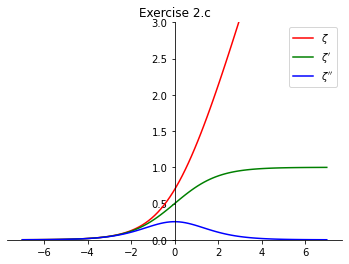
\includegraphics[width=.5\linewidth]{fig/exercise_2c.png}
	\caption{Plot of the $\zeta(z)$ function and its derivatives}
\end{figure}

Compute the asymptotes for $z \rightarrow \pm \infty$.
\begin{align*}
	\lim_{z \rightarrow + \infty} \zeta(z) &= \lim_{z \rightarrow + \infty} - \log \Big(\frac{1}{1+e^{\infty}}\Big) && \\
	&= \lim_{z \rightarrow + \infty} - \log \Big(\frac{1}{\infty}\Big) && \\
	&= \lim_{z \rightarrow + \infty} - \log(0) && \\
	&= \doubleunderline{\infty}
\end{align*}
\begin{align*}
	\lim_{z \rightarrow - \infty} \zeta(z) &= \lim_{z \rightarrow - \infty} - \log \Big(\frac{1}{1+e^{-\infty}}\Big) && \\
	&= \lim_{z \rightarrow - \infty} - \log \Big(\frac{1}{1+0}\Big) && \\
	&= \lim_{z \rightarrow - \infty} - \log(1) && \\
	&= \doubleunderline{0}
\end{align*}

\subsection{Task (d)}
Implement the sigmoid function in a Jupyter Notebook. Make it work such that you can
pass numpy arrays of arbitrary shape and the function is applied element-wise. Plot the
sigmoid function and its derivative by using matplotlib. 

\begin{figure}[tbh]
	\centering
	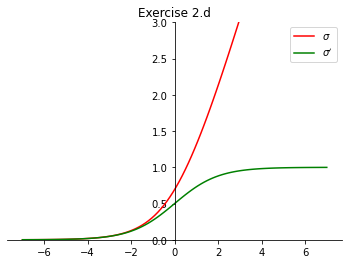
\includegraphics[width=.5\linewidth]{fig/exercise_2d.png}
	\caption{Plot of the $\sigma(z)$ function and its derivative}
\end{figure}

\subsection{Task (f)}
Show that $c_1(x) = (\sigma(x) -1)^2$ is non-convex.

\begin{align*}
	c_1^{\prime}(x) &= 2(\sigma(x)-1)\sigma(x)(1-\sigma(x)) && \\
	&= 2\sigma(x)(\sigma(x)-1)(1-\sigma(x)) && \\
	&= 2\sigma(x)(\sigma(x) - \sigma(x)^2 -1 + \sigma(x)) && \\
	&= 2\sigma(x)(-\sigma(x)^2 + 2\sigma(x) - 1) && \\
	&= -2\sigma(x)(\sigma(x)^2 -2\sigma(x) + 1) && \\
	&= -2\sigma(x)(\sigma(x) - 1)^2 && \\
	\\
	c_1^{\prime\prime}(x) &= -2\frac{d}{dx}\Big[\sigma(x)(\sigma(x) -1)^2\Big] && \\
	&= -2\Big[\sigma(x)(1-\sigma(x))(\sigma(x)-1)^2 + \sigma(x)2(\sigma(x) - 1)(-1)\sigma(x)(1-\sigma(x))\Big] && \\
	&= -2\sigma(x)(1-\sigma(x))(\sigma(x) - 1)\Big[2\sigma(x) +(\sigma(x)-1)\Big] && \\
	&= 2\sigma(x)(\sigma(x)-1)^2\Big[3\sigma(x)-1\Big] && \\
	&= \sigma(x)(\sigma(x)-1)^2(6\sigma(x)-2) && \\
\end{align*}

\subsection{Task (g)}
Compute the first and second derivative of the cross entropy function with respect to $w \in \mathcal{R}$ and for given $y \in {0,1}$. Show that $c_2$ is convex for $x \neq 0$.
\begin{align*}
	c_2(x) &= -(y \log(\sigma(w \cdot x)) + (1-y)\log(1-\sigma(w \cdot x))) && \\
	\\
	c_2^{\prime}(x) &= (-1) \frac{d}{dw} \Big[y \log(\sigma(w \cdot x)) + (1-y)\log(1-\sigma(w \cdot x))\Big] && \\
	&= (-1) \Big[y \frac{1}{\sigma(w \cdot x)} \sigma^\prime(w \cdot x) x - (1-y) \frac{1}{(1-\sigma(w \cdot x))} \sigma^\prime(w \cdot x) x\Big] && \\
	&= (-1) \sigma^\prime(w \cdot x)x\Big[\frac{y}{\sigma(w \cdot x)} - \frac{(1-y)}{(1-\sigma(w \cdot x))} \Big] && \\
	&= (-1) \sigma^\prime(w \cdot x)x\Big[\frac{y (1-\sigma(w \cdot x)) - (1-y)\sigma(w \cdot x)}{\sigma(w \cdot x)(1-\sigma(w \cdot x))}\Big] && \\
	&= (-1) \sigma^\prime(w \cdot x)x\Big[\frac{y (1-\sigma(w \cdot x)) - (1-y)\sigma(w \cdot x)}{\sigma^\prime(w \cdot x)}\Big] && \\
	&= -x \Big[y (1-\sigma(w \cdot x)) - (1-y)\sigma(w \cdot x)\Big] && \\
	&= -x \Big[y - y\sigma(w \cdot x) - \sigma(w \cdot x) + y\sigma(w \cdot x)\Big] && \\
	&= -x \Big[y - \sigma(w \cdot x)\Big] && \\
	&= x \Big[\sigma(w \cdot x) - y\Big] && \\
	\\
	c_2^{\prime\prime} &= \frac{d}{dw} \Big[x \cdot (\sigma(w \cdot x) - y)\Big] && \\
	&= x^2 \cdot \sigma^\prime(w \cdot x) && \\
	&= x^2 \sigma(w \cdot x) \sigma(1 - \sigma(w \cdot x))
\end{align*}

\section{Exercise 4: Review Question}
\begin{enumerate}[label=(\alph*)]
	\item It is beneficial because the input features are scaled similarly and thus build a loss landscape that is easier to optimize. Otherwise, the model additionally needs to learn to cope with the different feature scales, which leads to longer training and poorer performance.
	\item In machine learning, the learning problem can be formulated as an optimization problem, where the goal is to find the best fitting parameters. Thus optimization algorithms can be used.
	\item Gradient descent can be applied to all problems where a gradient with respect to the parameter to optimize can be computed. It will lead to a unique solution when the problem is convex. Thus the local minimum is also the global minima.
	\item The MSE cost with sigmoid as activation function is not convex for classification problems. This can lead to bad local minima.
	\item Then the optimization fails to converge to a minimum and oscillates around it.
	\item This phenomenon is called overfitting, where the model learns the parameter to fit the training dataset optimally. This will lead to poor generalization, and thus the training error will decrease whilst the testing increases.
	\item It is harder to reach a small train error because the dataset incorporates more variance. But it is easier to have a smaller generalization error when having a larger dataset since it is assumed that the dataset gets more similar to the true underlying distribution.
\end{enumerate}
\end{document}

